\subsection{playerState}
\label{ss:playerState}

\begin{figure}
	\centering
	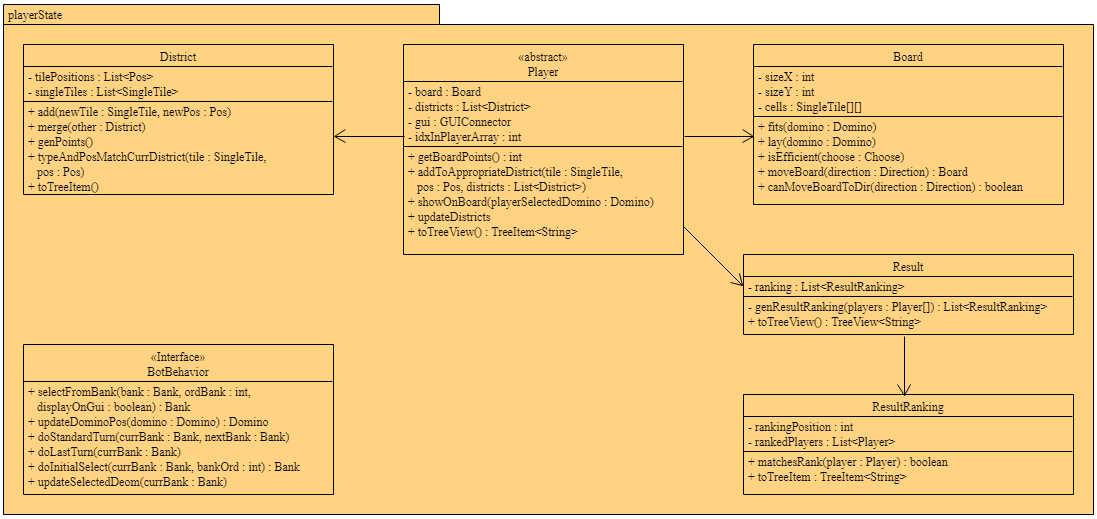
\includegraphics[width=\linewidth]{pics/playerStatePackage}
	\caption{UML-Darstellung des playerState packages}
	\label{fig:playerStatePackage}
\end{figure}

\import{programmierhandbuch/grundlegendeKlassen/playerState/district/}{districtClassDoc.tex}
\import{programmierhandbuch/grundlegendeKlassen/playerState/board/}{boardClassDoc.tex}
\import{programmierhandbuch/grundlegendeKlassen/playerState/botbehavior/}{botbehaviorClassDoc.tex}
\import{programmierhandbuch/grundlegendeKlassen/playerState/result/}{resultClassDoc.tex}
\import{programmierhandbuch/grundlegendeKlassen/playerState/resultRanking/}{resultRankingClassDoc.tex}
